\chapter{Deep}

\subsection{Deep Reinforcement Learning}\label{S:WDQN}
In the last few years, value-based \gls{rl} algorithms exploiting deep neural networks for $Q$-function approximation proved to be a very powerful way to solve complex highly dimensional \glspl{mdp}. The most famous algorithm is the Deep $Q$-Learning algorithm~\cite{mnih2015human}, more known as \gls{dqn} algorithm, where the $Q$-function is approximated with a deep neural network in an online setting. \gls{dqn} consists of a neural network to be trained online and another one that builds the target of the previous one. The target network is used for stability reasons, and it is updated with the weights of the online network every time a specified number of samples have been collected. The algorithm updates the online network using minibatch of samples collected using a $\varepsilon$-greedy policy, and stored in a replay memory, minimizing a loss function between the current estimate of the target network and the following target:
$$\hat{Q} =
  \begin{cases}
    r_t & \text{if $s_{t+1}$ is an absorbing state} \\
    r_t + \gamma \max_{a'} \hat{Q}(s_{t+1}, a'; \theta^-) & \text{otherwise}
  \end{cases}.
$$
where $\theta^-$ are the parameters of the target network. The overestimation problem caused by \gls{me} happens also in \gls{dqn} and results in critical loss of performance in some problems due to instability. The \gls{ddqn} algorithm~\cite{hasselt2015double} replaces \gls{me} with \gls{de} and shows considerable improvements and performance and stability.

\paragraph{Weighted Deep Q-Network} The replacement of \gls{me} with \gls{we} is not straightforward in this case due to difficulties in computing the variance of the approximation. The \gls{gp} regression, used in \gls{wfqi}, is commonly not used in \gls{drl} and a deep neural network adapts better in important \gls{drl} problems, such as the well known Atari domain. The estimation of mean and variance with a neural network is possible, but the computational complexity increases with the number of parameters such that it becomes unfeasible in deep neural networks. We propose to estimate the variance of the approximation using an ensemble of target networks, following the neural network architecture proposed in another algorithm called \gls{bdqn}~\cite{osband2017deep}. This work follows the \gls{dqn} algorithm described in~\cite{mnih2015human} with few, but important changes. The output of the neural network is split in $K$ heads that share the same first hidden layers. To perform bootstrapping, a binary mask $w_1, \dots, w_K \in {0,1}$ is assigned to each sample to indicate the heads assigned to it. The binary mask is generated with a binomial distribution with probability $p$. The exploration policy of \gls{bdqn} uniformly samples a head at the beginning of the episode, and follow the greedy policy learned by it. During the learning phase, the different heads are updated following the update rule of \gls{ddqn} to avoid the overestimation problem.

We propose to use the architecture of \gls{bdqn} replacing the \gls{de} with \gls{we} and to approximate the weights of its update formula using the output of each head. The resulting update formula is:
\begin{equation}
Q_{t+1}^k \leftarrow Q_t^k + r_t + \gamma \sum_{i \in {1, \dots, \#\mathcal{A}}} w_t^i Q_t^k(s_{t+1}, a_i; \theta_k^-),
\end{equation}
where $w_t^i$ is the weight of \gls{we} for action $i$ at time $t$ and $\theta_k^-$ are the parameters of the target network of the head $k$. Since the $Q$-values of the next state are computed using the target network, we propose to compute the weights using the online network in order to emulate the desirable behavior of \gls{de}. Note that the weights vector $\mathbf{w}_t = \langle w_t^1, w_t^2, \dots, w_t^K \rangle$ is the same for all heads.
The resulting algorithm is a slight change to the original \gls{bdqn} that allows to use the \gls{we} in the \gls{dqn} framework without differences in computational time and memory requirements w.r.t. \gls{bdqn}. We call this algorithm \gls{wdqn}.

\subsection{Deep Reinforcement Learning Scenario}
\subsubsection{Acrobot}
\begin{figure*}[t]
  \centering
  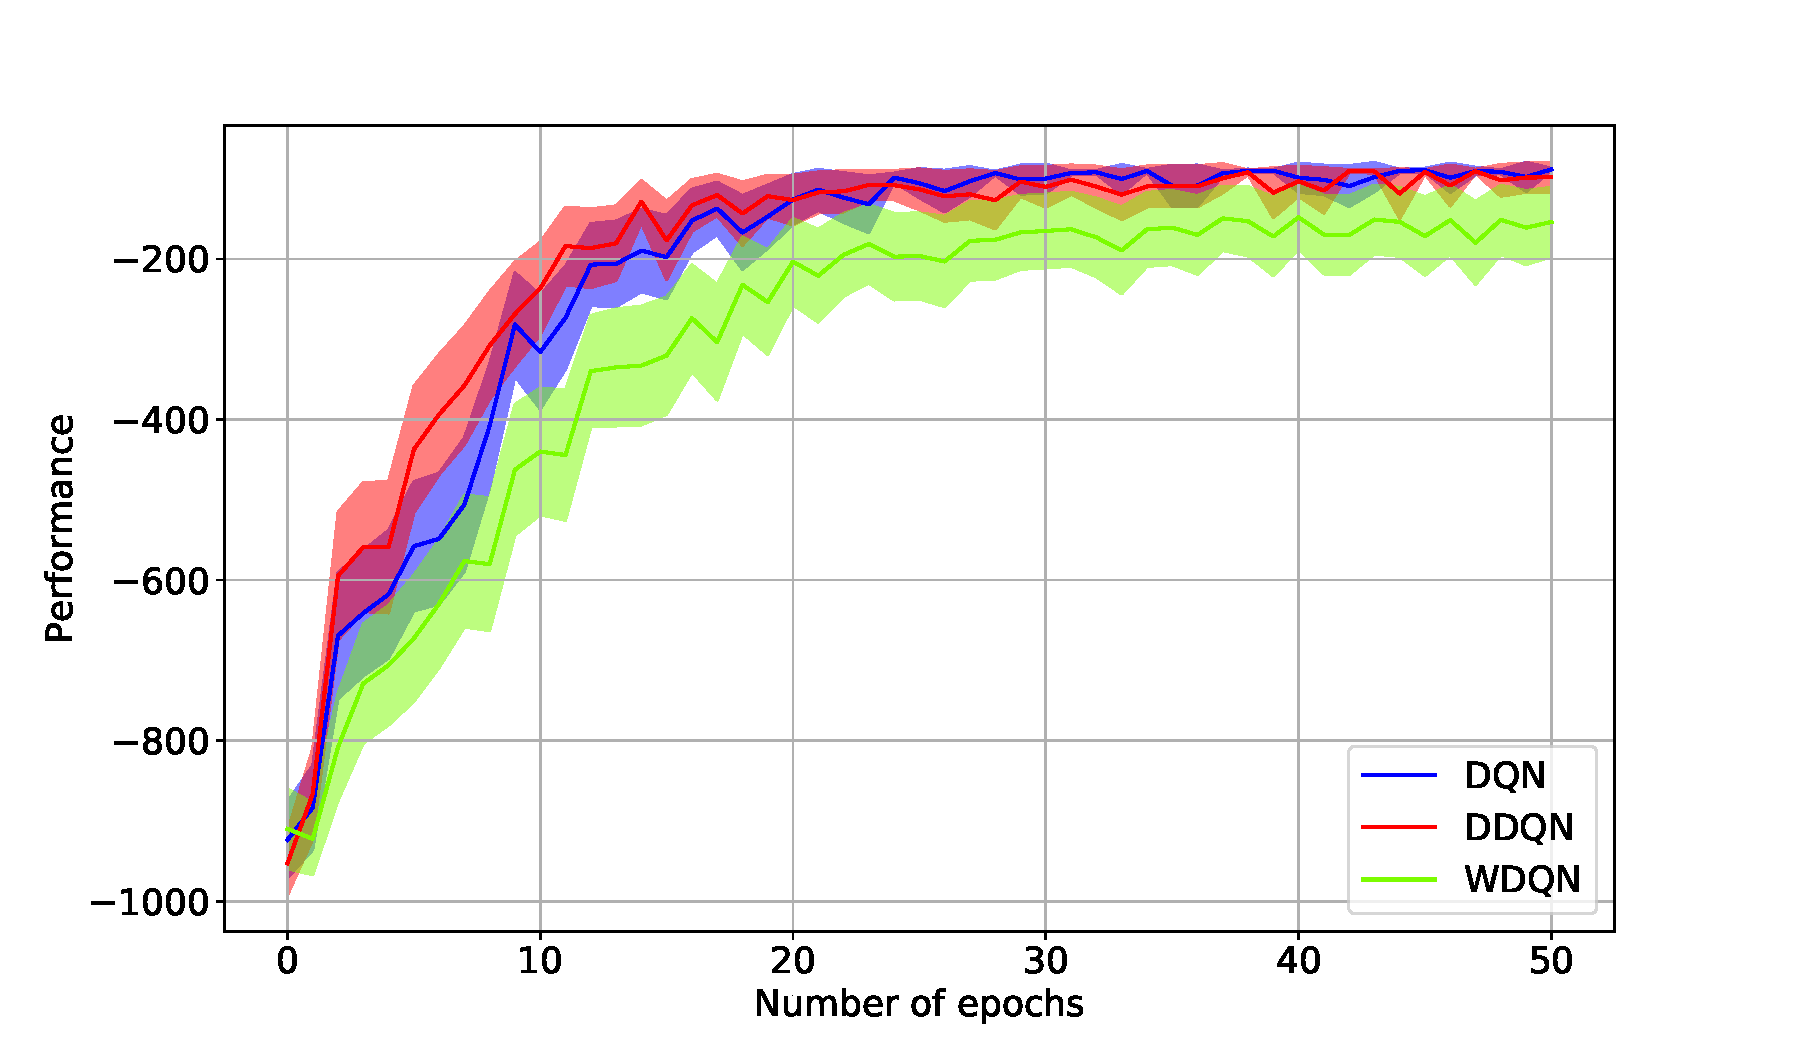
\includegraphics[scale=.6]{./img/acrobot.pdf}
  \caption{Average reward averaged on 10 experiments.
  }
  \label{F:acrobot}
\end{figure*}
\begin{table*}[t]
 \centering
 \caption{Average reward in continuous action MDP.}
 \label{T:acrobot_pars}
\begin{small}
\setlength{\tabcolsep}{4pt}
 \begin{tabular}{|c|c|}
\hline
Replay memory size & 50000\\
\hline
Initial replay size & 5000\\
\hline
Agent history length & 1\\
\hline
Target network update frequency & 100\\
\hline
Masking probability $p$ & $\nicefrac{2}{3}$\\
\hline
Number of hidden layers & 2\\
\hline
Number of neurons & 80\\
\hline
Number of heads & 10\\
\hline
Test samples & 5000\\
\hline
Evaluation frequency & 5000\\
\hline
Max no-op actions & 0\\
\hline
Total number of steps & 250000\\
\hline
Optimizer & Adam\\
\hline
 \end{tabular}
 \end{small}
\end{table*}

We evaluate the performance of \gls{bdqn} with \gls{me} and \gls{de} and \gls{wdqn} on the \gls{rl} problem of Acrobot. This is a well-known problem consisting in swinging up a two-link robot over a certain threshold. The state space and the dynamics of the problem make it a complex \gls{mdp} to be solved\footnote{We use the Acrobot-v1 environment of the OpenAI Gym library~\cite{gym}.}. The reward of the \gls{mdp} is -1 at each step and 0 when the arm of the bot reaches the threshold height. The discount factor is $\gamma = 0.99$. The horizon is set to 200. The training phase policy is the Bootstrapped policy described in Section \ref{S:WDQN}, while the evaluation policy computes the best action through ensemble voting. The hyperparameters of \gls{dqn} are the same used in the Atari experiments in~\cite{osband2017deep}, except for the ones specified in Table \ref{T:acrobot_pars}. The policy used is the Bootstrapped policy used in~\cite{osband2017deep}, where at the beginning of an episode a head is chosen randomly and the greedy policy derived by that head is followed. In our setting, we choose a random head at each step instead at each episode in order to favor exploration.

Figure \ref{F:acrobot} shows that all algorithms converges to the same performance, but \gls{wdqn} achieves it considerably faster than the others. Moreover, the score obtained by \gls{wdqn} is more stable during the training epochs, showing that \gls{we} helps also to stabilize the learning which is an important issue in the \gls{drl} scenario.
